\section{Empirical Evaluation}
\label{sec:eval}

We implemented our technique in a prototype tool called \tool{} (BUSiness TEsting Rules),
and conducted two empirical studies using two open-source applications 
and one IBM proprietary application. In the first study, we compared
the effectiveness of \tool{} in covering business rules with 
a related technique that systematically explores search space 
without any guidance. In the second study, we investigated the efficiency
of both the techniques. After describing the experimental setup,
we present results of the two studies.

\begin{table}[t]
\caption{Subjects used in our empirical studies.}
\centering
{\scriptsize
\tabcolsep=3pt
\begin{tabular}{|l|l|r|r|r|r|}
\hline
\multicolumn{1}{|c|}{Subject} & \multicolumn{1}{|c|}{URL} & \multicolumn{1}{|c|}{Entities} & \multicolumn{1}{|c|}{Operations} & \multicolumn{1}{|c|}{Rules} & \multicolumn{1}{|c|}{Rule parts} \\
\hline \hline
Cebu-pacific & www.cebupacificair.com 		& 8  & 10 &  	 & 31 \\
jBilling 		 & www.jbilling.com 					& 10 & 10 &   	 & 26 \\
App 				 & \multicolumn{1}{|c|}{---}	& 12 & 13 &     & 20 \\
\hline \hline
\textbf{Total} & 													& 	 & 33 &     & 77 \\
\hline
\end{tabular}
}
\label{tab:subjects}
\end{table}


\subsection{Experimental Setup}

\subsubsection{Implementation}
\label{sec:impl}

We implemented \tool{} as an Eclipse plugin, where users can model business
rules in a syntax-directed editor with various features such as auto completion
and on-the-fly detection of syntax errors. \tool{} uses \choco{} constraint
solver~\cite{Choco} for checking the satisfiability of sequences.
Currently, \tool{} provides a limited support for set types, where the number
of elements in sets is limited to size two. Also, since \choco{} does not 
provide functionality for extracting unsatisfied core, we use a heuristic-based
implementation to extract the core. While checking whether a concrete sequence
is satisfiable, \tool{} starts with the last operation of the sequence and
performs backward analysis by handling each operation and their rule parts. Therefore, when
a composed formula is unsatisfiable, it can happen only due to some
constraint in the most recently analyzed rule part. If the rule part includes
multiple constraints, \tool{} further analyzes each individual constraint to identify
the exact constraint that resulted unsatisfiability. Next \tool{} uses
variables involved in the identified constraint to extract the complete
unsatisfied core. Note that \tool{} may not extract 
the minimal unsatisfied core, however, the extracted core is sufficient
to suggest candidate operations. In future work, we plan to improve the efficiency
of our implementation by exploring advanced algorithms for extracting unsatisfied core~\cite{Liffiton:2008:ACM}
and also leverage other constraint solvers~\cite{DeMoura:2008}. We
also plan to leverage Green~\cite{VisserGD12} to cache the results of constraints
for further increasing the performance of our tool.

To show the efficiency of \tool{}, we 
implemented another tool, called \exhaust{}, that systematically explores sequences
without any guidance. Similar to \tool{}, \exhaust{} also uses a queue $q$
to store sequences. Given an operation ${\cal O}$ and a rule target $r$, 
\exhaust{} initially creates a sequence $seq$ with ${\cal O}\ [r]$ and adds $seq$
to $q$. For each $seq$, \exhaust{} associates a list of entities, referred to as \subject{ilist}. 
Initially, \subject{ilist} includes input entities of ${\cal O}$.
Next, \exhaust{} dequeues a sequence $qseq$ from $q$, removes an entity from its \subject{ilist},
and identifies all operations \{${\cal O}_1, {\cal O}_2, \ldots, {\cal O}_n$\}
that either create or modify that entity. \exhaust{} creates new sequences 
by adding each ${\cal O}_i$ to $qseq$. Also, if an ${\cal O}_i$ requires additional
input entities, it adds those entities to the \subject{ilist} corresponding to its newly
created sequence. Next, it adds all these newly created sequences to $q$
and repeats the process. Whenever \exhaust{} encounters a concrete sequence,
\ie{} sequence whose \subject{ilist} is empty, it uses \choco{} to check whether
the sequence is satisfiable. If yes, it returns the sequence; otherwise, continues
analyzing other sequences in the queue. \exhaust{} repeats this process until 
it finds a satisfiable sequence or it explores user-defined number of concrete
sequences. Being an unguided technique, \exhaust{} helps evaluate
the effectiveness of leveraging unsatisfied core as a guidance for searching
the desired sequence.

\subsubsection{Subjects and Rules}

We used two open-source applications and one IBM proprietary application, listed
in Table~\ref{tab:subjects}, as experimental subjects. Due to confidentiality reasons,
we refer to the proprietary application as \subject{App}. \subject{Cebu-pacific} is
an airlines application, \subject{jBilling} is an enterprise billing application,
and \subject{App} is a telecom application. Column~2 shows URL of each subject.
Columns~3--6 show additional details such as number of entities, operations,
and rules. For each subject, we identified a module that is likely to have large
number of interesting rules with respect to test data, and modeled those modules using our tool. In particular,
we used \textit{ticket cancellation} and \textit{generate invoice} modules for \subject{Cebu-pacific} and 
\subject{jBilling}, respectively. Overall, we modeled $33$ operations with $XX$ rules and
$77$ rule parts.\footnote{The complete dataset including the models and the generated
test sequences is available at \url{http://tinyurl.com/k4b4j8x} (also available on request
from the authors).}

\subsubsection{Method}

We applied both \tool{} and \exhaust{} on models created for each subject and generated
test sequences. For each rule part, we let each tool explore up to a maximum of $100$
concrete sequences. Next, we inspected generated sequences to ensure that 
they cover respective rule parts. To study the efficiency of both the tools, we measured the number of sequences
explored and also measured lengths of sequences produced by each tool.
All experiments were conducted on an Intel Core 2 Duo CPU
machine with 2.53 GHz and 8GB RAM. Next, we present the results of the studies.

\subsection{Coverage of Business Rules}

\begin{figure}[t]
\centering
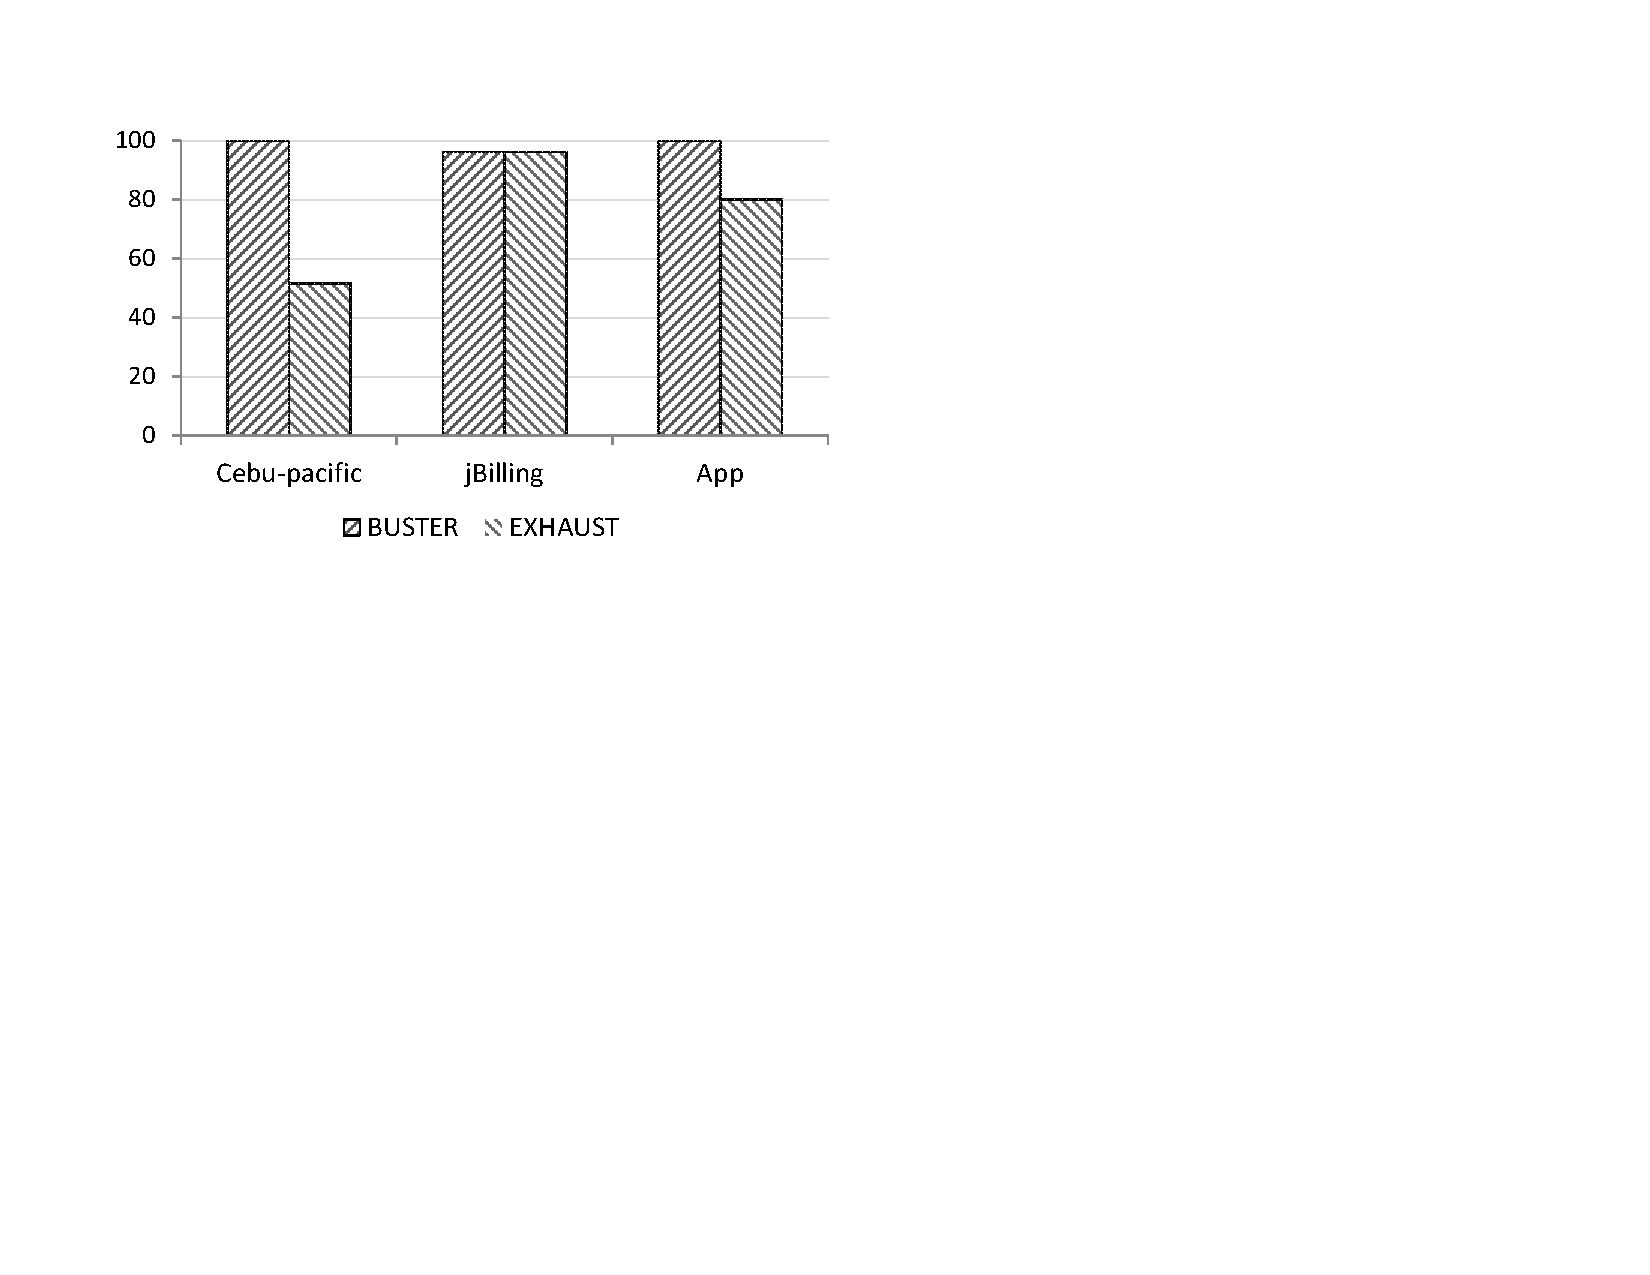
\includegraphics[width=0.7\columnwidth, clip, trim = 18mm 120mm 140mm
  18mm]{figs/Study-1.pdf}
\caption{Effectiveness of the two techniques in covering business rules.}
\label{fig:effectiveness}
\end{figure}

Figure~\ref{fig:effectiveness} shows the results for all three subjects. 
In the figure, x axis shows subjects, whereas y axis shows percentages of rule parts
covered by each tool. For example, for \subject{Cebu-pacific},
\tool{} generated desired sequences for all $31$ rule parts, whereas \exhaust{} was able
to generate sequences only for $16$ rule parts. Overall, the results show 
that \tool{} handled $99$\% of rule parts, whereas \exhaust{}
handled only $74$\% of rule parts.

While analyzing our results, we identified that the rule parts that were 
not covered by \exhaust{} require complex sequences. In particular, \exhaust{}
could handle subjects such as \subject{jBilling}, where there are only a few
operations that create or modify each entity. On the other hand, it could not
handle subjects such as \subject{Cebu-pacific}, where there are several operations
that modify the same entity. Both \tool{} and \exhaust{} could not cover 
one rule part in \subject{jBilling} due to an issue with \choco{} solver. \choco{} produced
out of memory error while solving the composed formula for that rule part. We next present a complex sequence
generated by \tool{} for a rule part in \subject{Cebu-pacific}. This rule part is
related to refunding money to the passenger because of cancellation of flight due
to a delay of more than two hours.

{\scriptsize
\begin{alltt}
 int fund = 200, passenger = 1;
 CreateFund(fund, passenger, out: Fund fund);
 CreateTicket(passenger, out: Ticket ticket);
 int flight = 901, price = 100, departure = 10; 
 MakeSector(flight, price, out: Sector sector);
 AddSector(ticket, sector, fund,  
                out: Ticket ticket1, out: Fund fund1);
 int delay = 3, sectorid = 1; 
 DelayFlight(ticket1, sectorid, delay, out: Ticket ticket2);
 PartialCancellation(ticket2, sectorid, out: Ticket ticket3);
 Refund(ticket3, sectorid, fund1, 
                out: Ticket ticket4, out: Fund fund2);
\end{alltt}
}

\subject{Cebu-pacific} allows booking a ticket as multiple sectors, 
where each sector represents part of the journey from one city to another city. The airlines
has a refund policy where if the flight corresponding to any sector gets canceled
due to a delay of more than two hours, passengers can get refund so as to make alternate
travel arrangements. To cover this rule part that belongs to the operation
\subject{Refund}, a specific instance of \subject{Ticket} entity
is required. First, the ticket should include at least one sector and the passenger
should have sufficient funds to add a sector to the ticket. Next, the flight corresponding
to that sector should be delayed by more than two hours, and hence should be canceled
due to significant delay. \tool{} was able to successfully generate the preceding sequence,
whereas \exhaust{} was not able to generate any sequence for this rule part.
Overall, our results show promising benefits of our technique in effectively generating
complex sequences for covering business rules.

\begin{table}[t]
\caption{Efficiency of \tool{} and \exhaust{}.}
\centering
{\scriptsize
\tabcolsep=3pt
\begin{tabular}{|l|r|r|r|r|r|r|r|r|}
\hline
& \multicolumn{4}{|c|}{Sequence Length} & \multicolumn{4}{|c|}{\# of Sequences Explored} \\
\cline{2-9}
& \multicolumn{2}{|c|}{\tool{}} & \multicolumn{2}{|c|}{\exhaust{}} & \multicolumn{2}{|c|}{\tool{}} & \multicolumn{2}{|c|}{\exhaust{}}  \\
\cline{2-9}
\multicolumn{1}{|c|}{Subject} & \multicolumn{1}{|c|}{Max} & \multicolumn{1}{|c|}{Avg} & \multicolumn{1}{|c|}{Max} & \multicolumn{1}{|c|}{Avg} & \multicolumn{1}{|c|}{Max} & \multicolumn{1}{|c|}{Avg} & \multicolumn{1}{|c|}{Max} & \multicolumn{1}{|c|}{Avg} \\
\hline \hline
Cebu-pacific 	 &  7		& 5 &  9 &  5	 &  27 &  4	&  100 & 73 \\
jBilling		 	 &  6		& 3 &  6 &  3	 &  48 &  2	&  39  &  2 \\
App					 	 &  9		& 6 & 10 &  6	 &  51 &  5	& 100  & 46 \\
\hline
\end{tabular}
}
\label{tab:stats}
\end{table}

\subsection{Efficiency}

Table~\ref{tab:stats} shows data about lengths of sequences and number 
of sequences generated by both the tools. Columns~2--5 show the maximum 
and average lengths of sequences generated for all rule parts. 
On the other hand, Columns~6--9 show the number of 
sequences explored by each technique for all rule parts. 

Our results show that \tool{} generated relatively shorter sequences
compared to \exhaust{}. Furthermore, on average, \tool{} explored
only a few sequences compared to \exhaust{}. For example,
for \subject{Cebu-pacific}, \tool{} explored an average of $4$ sequences
(maximum of $27$), whereas \exhaust{} explored an average of $73$ sequences
for each rule part. Overall, the results show that \tool{} is highly efficient
compared to \exhaust{}.
